\documentclass[13pt,oneside]{book}
\usepackage[utf8]{inputenc}
\usepackage{url}
\usepackage{graphicx}

\usepackage{geometry}
\geometry{a4paper, left=20mm, right=20mm, top=20mm, bottom=20mm}
\usepackage[margin=1.2in]{geometry}
\usepackage[toc,page]{appendix}
\usepackage{graphicx}
\usepackage{natbib}
\usepackage{lipsum}
\usepackage{caption}

\begin{document}

\captionsetup[figure]{margin=1.5cm,font=small,labelfont={bf},name={Figure},labelsep=colon,textfont={it}}
\captionsetup[table]{margin=1.5cm,font=small,labelfont={bf},name={Table},labelsep=colon,textfont={it}}
\setlipsumdefault{1}

\begin{titlepage}
\begin{center}
{\LARGE College Of Engineering Trivandrum}\\[3cm]
\linespread{1.2}\huge {\bfseries Application Software Development Lab}\\[3cm]
\linespread{1}

\includegraphics[width=5cm]{img/emblem.jpeg}\\[3cm]
{\Large GOKUL K\\ S5  CSE \\ Roll No:21\\ TVE18CS021 }\\[1cm]


\textit{ }\\[2cm]
Department of Computer Science\\[0.2cm]
\today
\end{center}

\end{titlepage}

\newpage

\begin{frame}{}
    \centering
    \hspace*{-0.5cm}
    $\vcenter{\hbox{
\includegraphics[width=1.5cm]{img/emblem.jpeg}}}$
    $\vcenter{\resizebox{0.95\textwidth}{!}{
        \begin{tabular}{c}
             CS333 - Application Software Development Lab $\cdot$ 2020 $\cdot$   \\
             \hline 
        \end{tabular}
    }}$
\end{frame}
\section*{Cycle 1}
\section*{Expt 3}
\begin{center}
    \Large{Basic SQL Queries - II}
\end{center}

\section*{Aim}
\large{Understand basic SQL queries
\begin{enumerate}
	\item ALTER
	\item RENAME
	\item SELECT DISTINCT
	\item SQL IN
	\item SQL BETWEEN
	\item SQL ALIASES
	\item SQL AND
	\item SQL OR
\end{enumerate}
}

\section*{Experiment}
	\begin{enumerate}
\item
Create a CAR database with the following details.
\begin{verbatim}

	+----+--------+------------+---------+-------------+
	| id | name   | company    | country | approxprice |
	+----+--------+------------+---------+-------------+
	|  1 | Beat   | Chevrolet  | USA     |         4.0 |
	|  2 | Swift  | Maruti     | Japan   |         6.0 |
	|  3 | Escort | Ford       | USA     |         4.2 |
	|  4 | Sunny  | Nissan     | Japan   |         8.0 |
	|  5 | Beetle | Volkswagen | Germany |        21.0 |
	|  6 | Etios  | Toyota     | Japan   |         7.2 |
	|  7 | Sail   | Chevrolet  | USA     |         5.0 |
	|  8 | Aria   | Tata       | India   |         7.0 |
	|  9 | Passat | Volkswagen | Germany |        25.0 |
	| 10 | SX4    | Maruti     | Japan   |         6.7 |
	+----+--------+------------+---------+-------------+
\end{verbatim}
 
Syntax:
\begin{verbatim}
CREATE TABLE CAR(
        id INT PRIMARY KEY,
        name VARCHAR(10),
        company VARCHAR(20),
        country VARCHAR(10),
        approxprice DECIMAL(1, 3)
);
INSERT INTO CAR 
VALUES
        (1, 'Beat', 'Chevrolet', 'USA', 4),
        (2, 'Swift', 'Maruti', 'Japan', 6),
        (3, 'Escort', 'Ford', 'USA', 4.2),
        (4, 'Sunny', 'Nissan', 'Japan', 8),
        (5, 'Beetle', 'Volkswagen', 'Germany', 21),
        (6, 'Etios', 'Toyota', 'Japan', 7.2),
        (7, 'Sail', 'Chevrolet', 'USA', 5),
        (8, 'Aria', 'Tata', 'India', 7),
        (9, 'Passat', 'Volkswagen', 'Germany', 25),
        (10, 'SX4', 'Maruti', 'Japan', 6.7);

\end{verbatim}
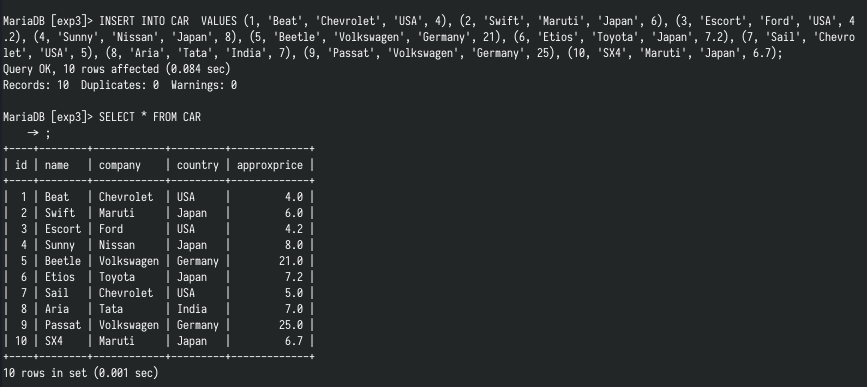
\includegraphics[]{img/p3/ss1.png}


\item
List the car companies in the database.
 
Syntax:
\begin{verbatim}
SELECT company 
FROM CAR;

\end{verbatim}
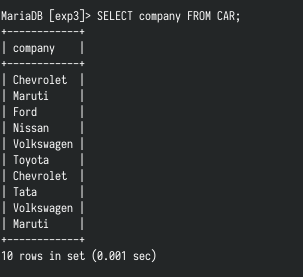
\includegraphics[]{img/p3/ss2.png}


\item
List the names of countries with car production companies.
 
Syntax:
\begin{verbatim}
SELECT country 
FROM CAR;

\end{verbatim}
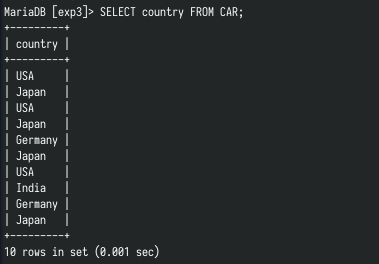
\includegraphics[]{img/p3/ss3.png}


\item
List the details of cars within a price range 4 to 7 lakhs.
 
Syntax:
\begin{verbatim}
SELECT *
FROM CAR
WHERE approxprice>4 AND approxprice<7;

\end{verbatim}
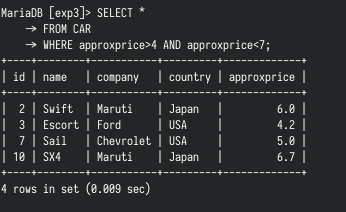
\includegraphics[]{img/p3/ss4.png}


\item
List the name and company of all the cars originating from India and
 having price <= 8 lakhs.
 
Syntax:
\begin{verbatim}
SELECT name, company
FROM CAR
WHERE country='India' AND approxprice<=8;

\end{verbatim}
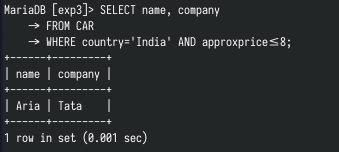
\includegraphics[]{img/p3/ss5.png}


\item
List the names, companies and countries of cars either from Nissan or
 from Germany.
 
Syntax:
\begin{verbatim}
SELECT name, company, country
FROM CAR
where company='Nissan' OR country='Germany';

\end{verbatim}
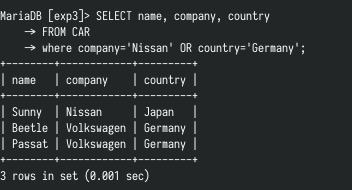
\includegraphics[]{img/p3/ss6.png}


\item
List the names of all cars produced by (Maruti,Ford). Use SQL IN
 statement.
 
Syntax:
\begin{verbatim}
SELECT name
FROM CAR
WHERE company IN ('Maruti', 'Ford');

\end{verbatim}
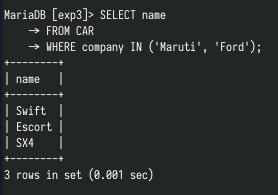
\includegraphics[]{img/p3/ss7.png}


\item
Alter the table cars to add a new field year (model release year). Update
 the year column for all the rows in the database.
 
Syntax:
\begin{verbatim}
ALTER TABLE CAR
ADD COLUMN year INT;
UPDATE CAR
SET year=2010;

\end{verbatim}
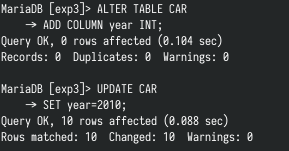
\includegraphics[]{img/p3/ss8.png}


\item
Retrieve the names of all cars and display names under 'Car\_name'.
 
Syntax:
\begin{verbatim}
SELECT name AS 'Car_name'
FROM CAR

\end{verbatim}
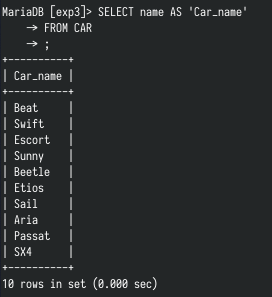
\includegraphics[]{img/p3/ss9.png}


\item
Rename the attribute name to car\_name.
 
Syntax:
\begin{verbatim}
ALTER TABLE CAR
CHANGE COLUMN name Car_name VARCHAR(10);

\end{verbatim}
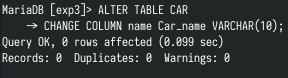
\includegraphics[]{img/p3/ss10.png}


\item
List the car manufactured by Toyota (to be displayed as cars\_Toyota).
 
Syntax:
\begin{verbatim}
SELECT Car_name AS 'cars_Toyota'
FROM CAR
WHERE company='Toyota';

\end{verbatim}
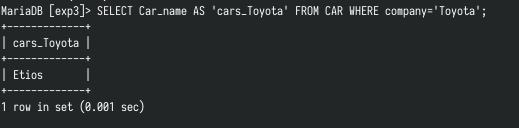
\includegraphics[]{img/p3/ss11.png}


\item
List the details of all cars in alphabetical order.
 
Syntax:
\begin{verbatim}
SELECT *
FROM CAR
ORDER BY Car_name ASC;

\end{verbatim}
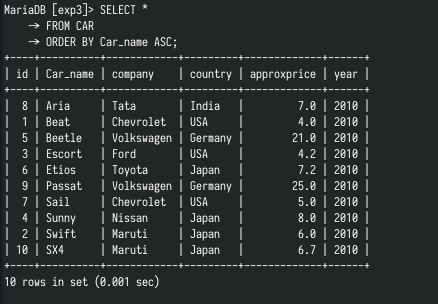
\includegraphics[]{img/p3/ss12.png}


\item
List the details of all cars from cheapest to costliest.

Syntax:
\begin{verbatim}
SELECT *
FROM CAR
ORDER BY approxprice ASC;

\end{verbatim}
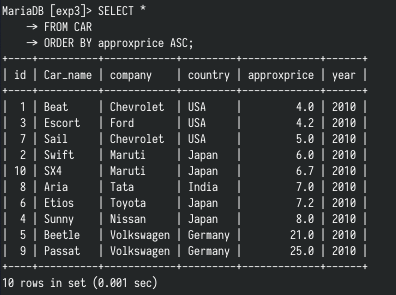
\includegraphics[]{img/p3/ss13.png}
	\end{enumerate}
	\section*{Result}
	The basic SQL for creating and modifying a table is executed and their output
	is verified in a MySQL environment.
\end{document}